\section{Lecture 1}
% introduction to sensor fusion 
% examples of sensor fusion 
% problem of finding position of an object with inertial sensors 
% integration drift 
% human motion capture 
% sensor fusion model 
\subsection{Sensor fusion}
The first part of the course covers the identification of static models based on output data and filtering to estimate the state of a system through time. An application that is closely related to these topics is sensor fusion. Sensor fusion is the process of using different sensors to obtain more information about a quantity, which could've been obtained from just one sensor. THis is done to get better estimates and information about that quantity. Some examples of sensor fusion include: 
\begin{itemize}
	\item Motion capture of a ice skater.
	\item Motion capture of the actor playing Ted.
	\item Sensors on a drone to find the position and orientation. 
\end{itemize} 
An important problem is the issue of find the information on the exact position and orientation of an object as it moves through time. Theoretically, the figure below shows how this can be done by using inertial sensors that measure angular acceleration and linear acceleration. 
\begin{figure}[H]
	\centering 
	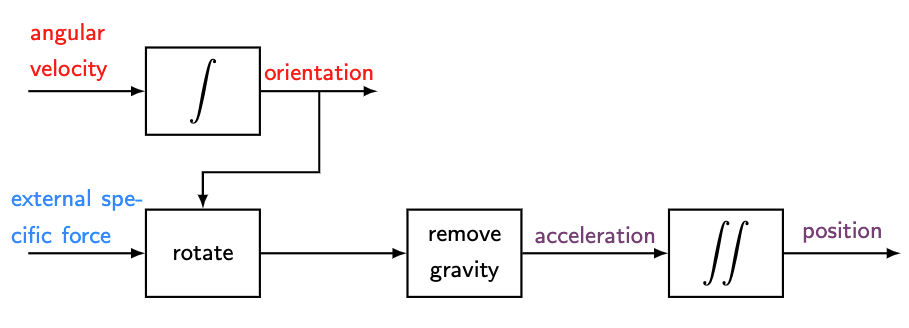
\includegraphics[scale = 0.4]{Lecture 1/images/inertial sensors}
	\caption{Process to obtain position and orientation of an object}
	\label{inertial sensors}
\end{figure}
The problem with this apporach is that since integration is involved, any errors, no matter how small, will eventually get summed up and lead to large errors in the position of the object. This phenomenon is called \emph{integration drift}. To prevent such an eventuality, more information is needed about the system. This can be provided through additional sensors, information about the operation of the sensor itself or physical knowledge about the system. An example of how this can be done is seen in the following example. 
\begin{figure}[H]
	\centering 
	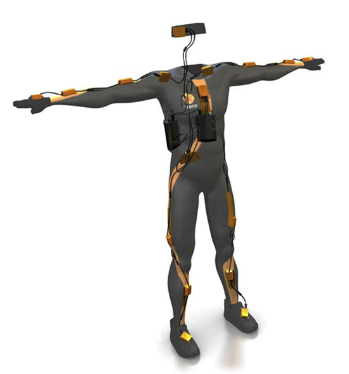
\includegraphics[scale = 0.4]{Lecture 1/images/motion capture}
	\caption{Example of sensor fusion}
	\label{motion capture}
\end{figure}
From the above setup there could a few issues that arise. The first as already discussed is the integration drift that might occur due to errors in measurement by the sensor. The second is that we have to assume that the sensors placed on the body are rigidly fixed in place when in reality that is not the case. Since the body is made of soft, deformable tissue, it is likely that the sensors have some relative motion with respect to the body. To counter some of these problems we can do the following: 
\begin{itemize} 
	\item Realise that the joints of the body are fixed in place and they have no relative motion with respect to the body. Adding this as a constraint to estimating the position of each limb would then lead to more realistic results. 
	\item Idefintiy parameters for the model that are currently unknown. How much to the sensors move by when a particular movement is executed? Could that be modeled? Could the bias in sensor be modelled by certain unknown parameters? 
\end{itemize} 
Soliving these problems would require the knowledge of both filtering technoiques and static model parameter identification.
\subsection{System identification} 
% definitions, art and science 
% white box system identification
% black box system identification
% parametric system identification
	% how to choose the parametric function to identify 
% prediciton error methods 
% subspace methods
Subspace identification is the process of finding mathematical models for dynamical systems based on input-output behavior of the system. There are two classes of the identification problem, which are white-box identification and black-blox identification.\\
\newline
With white box identification we are already aware of the differential equations behind the physical process. We can think of textbook examples of pendulum, mass-spring-damper systems, electrical ciruits to which we can apply newton's laws or kirchkoff's laws to find the mathematical model. However, in order to control the system and be precise, we also need to know the model parameters. These are things like mass, spring stiffness, resistance, voltage, etc. White box identification is then the science of looking at the input-output behaviour to identify these physical parameters.\\
\newline
There are also other kinds of systems for which we cannot write down a differential equation because either because they are too complex or there are many variables that affect the dynamics of the system. Black box identification then involves assuming a certain structure for the model of these systems and trying to find the parameters that best suit the input-output behavior. 
\subsection{Parametric system identification} 
Both the two cases above then have the following set up: You have input and output data given by $(u_{n}, y_{n})_{n = 1}^{N}$. We have a function $f(.,.,.|\theta)$ that we suspect models the system (black box), or know for sure it models the system (white box) and we have to identify the parameters in $\theta$ such that,
\begin{equation}
	y_{n} \approx \hat{y}_{n} = f(u, y, e|\theta)
\end{equation}
We see from the above, that $f$ can depend on past inputs and outputs. And are not neccesarily confined to just the previous input-output pair. 
The question then becomes: 
\begin{itemize}
	\item What kind of function should $f$ be? There are so many options. 
	\item Should $f$ be linear or non-linear? 
	\item How much data from the past should be part of $f$? 
\end{itemize}
\subsection{Linear system identification}
In this course, the focus will be on linear system identification. Under this there are two main approaches. 
\subsubsection{Prediction error methods}
For this method we assume that the input-output and error-output relationship can be modeled with transfer funcitons. They would take the form of, 
\begin{equation}
	\hat{y}_{n} = \hat{G}(q|\theta)u_{n} + \hat{H}(q|\theta)e_{n}
\end{equation}
Finding the parameters in $\theta$ would then require solving a non-linear optimisation problem. The problem is also likely to be non-convex which means there could be multiple local minima and the solution we obtain could largely depend on our initial guess. 
\subsubsection{Subspace methods}
For subspace methods, instead if system identification we use state space methods to model the system. Particular, this course will use the following formulation: 
\begin{align}
	x_{n+1} &= Ax_{n} + Bu_{n} + Ke_{n}\\
	y_{n} &= Cx_{n} + Du_{n} + e_{n}
\end{align}
The advantage of the subspace identification method is that solving a non-linear optimisation problem is not required. Just through the use of linear algebra (SVD decomposition, RQ factorisation) we can arrive at the (A, B, C, D) matrices and identify the system. 
\section{Math preliminaries}
\subsection{Some linear algebra revision}
We first consider the least squares problem which is 
\begin{equation}
	\min_{\theta} \epsilon^{\top}\epsilon \hspace{15mm} \text{Where,} \quad y = F\theta + \epsilon
	\label{least squares problem}
\end{equation}
$y$ is a vector of outputs, $F$ is the parameter matrix and $\theta$ is the parameter vector that is to be found. $\epsilon$ is the error between the model $F\theta$ and the true system behavior $y$. Suppose that, $y \in \mathbb{R}^{3}, F \in \mathbb{R}^{3 \times 2}, \theta \in \mathbb{R}^{2}$. 
\begin{equation}
	F = 
	\begin{bmatrix}
		f_{1} & f_{2}
	\end{bmatrix}
\end{equation}
where $f_{1}, f_{2} \in \mathbb{R}^{3}$. We can then visualise $F\theta$ as the linear combinations of the vectors $f_{1}, f_{2}$ and all the possible linear combinations would fill up an entire plane. The solution to the least squares problem is then to combine $f_{1}, f_{2}$ such that the resultant vector $\theta_{1}f_{1} + \theta_{2}f_{2}$ is the projection of the measurement vector $y$ onto the plane $F$. The figure below shows this visualisation. 
% include figure of geomteric representation of the least squares problem. 

There are some interesting properties of the solution to the least squares problem that is worth nothing. 
\begin{lemma}
	$F^{\top}F$ is a symmetric matrix and positive (semi-)definitie. 
\end{lemma}
To prove the above, we can first write out $F$ to be the following, 
\begin{equation}
	F = 
	\begin{bmatrix}
		f_{11} & f_{12} & \cdots & f_{1n}\\
		f_{21} & f_{22} & \cdots & f_{2n}\\
		\vdots & \vdots & \vdots & \vdots\\
		f_{m1} & f_{m2} & \cdots & f_{mn}
	\end{bmatrix}
	\hspace{10mm}
	F^{\top} = 
	\begin{bmatrix}
		f_{11} & f_{21} & \cdots & f_{m1}\\
		f_{12} & f_{22} & \cdots & f_{m2}\\
		\vdots & \vdots & \vdots & \vdots\\
		f_{1n} & f_{2n} & \cdots & f_{mn}
	\end{bmatrix}
\end{equation}
We then consider the first column and row of $F^{\top}F$, and compare the results. Multiplying from the left, we have the column picture, where we multiply the $F^{\top}$ with the first column of $F$.
\begin{equation}
	F^{\top}f_{1} = 
	\begin{bmatrix}
		f_{11}^{2} + f_{21}^{2} + \cdots + f_{m1}^{2}\\
		f_{11}f_{12} + f_{21}f_{22} + \cdots + f_{m1}f_{m2}\\
		\vdots\\
		f_{11}f_{1n} + f_{21}f_{2n} + \cdots + f_{m1}f_{mn}
	\end{bmatrix}
\end{equation}
We can then look at the row picture where multiply $F$ from the left with the first row of $F^{\top}$, 
\begin{equation}
	f_{1}^{\top}F = 
	\begin{bmatrix}
		f_{11}^{2} + f_{21}^{2} + \cdots + f_{m1}^{2} & f_{11}f_{12} + f_{21}f_{22} + \cdots + f_{m1}f_{m2} & \cdots & f_{11}f_{1n} + f_{21}f_{2n} + \cdots + f_{m1}f_{mn}
	\end{bmatrix}
\end{equation}
We observe that $(f_{1}^{\top}F)^{\top} = F^{\top}f_{1}$, extending this to all columns we can conclude that, 
\begin{equation}
	(F^{\top}F)^{\top} = F^{\top}F
\end{equation}
Which is the definition of a symmetric matrix. To see that $F^{\top}F$ is at the very least postive semi-definition, we go back to the definition of postive semi-definiteness, 
\begin{align}
	\text{If,} \hspace{10mm} A &\geq 0\\
	z^{\top}Az &\geq 0
\end{align}
If we take $A = F^{\top}F$, thwn we for positive semi-definitess we need to satisfy, 
\begin{align} 
	z^{\top}F^{\top}Fz &\geq 0\\
	\|Fz\|^{2}_{2} &\geq 0 
\end{align}
Which is certainly true, since we are talking about the 2-norm of a vector. We also know from the discussion we had earler that of $F$ is not full rank, there is no unique soltion for $\theta$ since the columns of $F$ that are linearly dependent do not contribute anything. That implies that $(F^{\top}F)^{-1}$ is not inverible and that $F^{\top}F$ is for sure positive semi-definite and has 0 as an eigenvalue. From the eigenvalue decomposition, we know that: 
\begin{equation}
	A = S\Omega S^{-1}
\end{equation}
Where, 
\begin{equation}
	\Omega = 
	\begin{bmatrix}
		\lambda_{1} & 0 & \cdots & 0\\
		0 & \lambda_{2} & \cdots & 0\\
		\vdots & \vdots & \ddots & \vdots\\
		0 & 0 & \cdots & \lambda_{n}
	\end{bmatrix}
\hspace{10mm} \text{Where,} \quad Ae_{i} = \lambda_{i}e_{i}
\end{equation}
If we again take $A = F^{\top}F$ and take the inverse, 
\begin{equation}
	(F^{\top}F)^{-1} = S\Omega^{-1}S^{-1}\\
\end{equation}
If there is a $\lambda_{i} = 0$ then $\Omega^{-1}$ would not exist which corresponds to the least squares problem having no solution. 
\subsection{Random variables and processes} 
A random variable $\theta$ is a variable whose values depend on a random phenomenon and can take on unpredictable values. There are fortunately some properties of random variables that allow us to work with them despite thier unpredictability. We usuually work with the \emph{expected} value of the random variable's properties.\\
\newline
Mean: We observe the random variable in $N$ number of experiments and record the values of $\theta$. Summing he values up and taking the average out of all the experiments provides the mean of the random variable $\theta$. 
\begin{equation} 
	E\Big[\theta \Big] = \frac{1}{N}\sum_{i = 1}{N} \theta_{i}
\end{equation}
Covariance: It is the measure of how spread out the values of theta are likely to be relative to the mean. The correct way to visualise this is to picture an ellipse where the size of the ellipse is a measure of covariance. The off diagnal terms play a role in shaping the matrix. 
\begin{equation}
	E\Big[ (\theta - \mu_{\theta})(\theta - \mu_{\theta})^{\top} \Big] = P_{\theta} = \frac{1}{N}\sum_{i = 1}^{N}(\theta_{i} - \mu_{\theta})(\theta_{i} - \mu_{\theta})^{\top}
\end{equation}
Correlation: It is a special case of the measure of covariance when the mean is zero. 
\begin{equation}
	E\Big[\theta \theta^{\top} \Big] = R_{\theta} = \frac{1}{N} \sum_{i = 1}^{N} \theta \theta^{\top}
\end{equation}
A random process $x(k)$ comprises of a collection of random variables $(k = 1, 2,..., N)$ after the completion of one experiement. In particular a random process is said to be stationary, if: 
\begin{itemize}
	\item The mean of $x(k)$ remains constant over the entire process. 
		\begin{equation}
			\mu_{x}(k) = \mu_{x}
		\end{equation}
	\item The auto-correlation function only depends on the lag between two random variables. 
		\begin{equation}
			R_{x}(k, l) = R_{x}(k - l) = R_{x}(\tau) = E\Big[x(k)x(k-\tau) \Big]
		\end{equation}
	\item The variance $E\Big[ (x(k) - \mu_{x})^{2}\Big]$ is finite. 
\end{itemize}
The difference between variance, covariance, auto-covariance, cross-covariance needs to be clarified. Variance applies to only the random variable itself (that is, $E\Big[ (x(k) - \mu_{x})^{2}\Big]$ while covariance is a measure of how the different components of the random variable depend on each other (shape of the ellipse) $E\Big[ (x(k) - \mu_{x})(x(k) - \mu_{x})^{\top}\Big]$. Auto-covariance is the measure of how the random variables depend on the lag between when they were measures (that is, $E\Big[ (x(k) - \mu_{x})(x(k - \tau) - \mu_{x})^{\top}\Big]$ and cross-covariance measure how two random variables depend on each other (that is, $E\Big[ (x(k) - \mu_{x})(y(k - \tau) - \mu_{y})^{\top}\Big]$.\\
\newline
A special kind of random process is the white noise signal. It has the property that it's mean is 0 and that the the signals at received at a certain time do not depend on the signals recieved at nother time. We can summarise the property of white noise signals as $e \backsim \mathcal{N}(0, \mathcal{I})$. 



















